\subsection{Princípio de Arquimedes}

O experimento realizado foi embasado no Princípio de Arquimedes, o qual afirma que um fluido exerce uma força ascendente em um corpo que se encontra mergulhado no mesmo fluido, sendo que o módulo dessa força corresponde ao peso do volume do líquido deslocado.

Assim, foi montado um dispositivo dentro do laboratório para verificar tal princípio, de modo que um pequeno cilindro fosse acoplado na extremidade inferior de uma mola posicionada verticalmente. Logo, quando o cilindro foi solto, seu peso (força gravitacional) deformou a mola até tal força se igualar com a força elástica proporcionada em função do tempo, enquanto uma régua posicionada verticalmente próximo à mola viabilizou a marcação da deformação.

\begin{figure}[H]
    \centering
    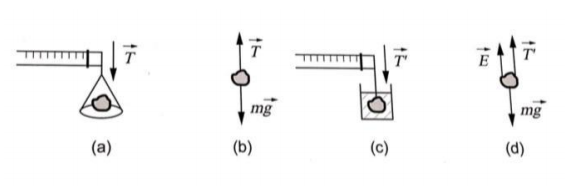
\includegraphics[scale=0.8]{images/Experimento1.png}
    \caption{Esquema de Forças atuando em uma balança de tração.}
\end{figure}

Dois casos foram realizados. O primeiro foi com o cilindro, sem submersão deste em um líquido, foi solto, enquanto o segundo houve submersão do corpo cilíndrico em um recipiente com água após ser solto.